\subsection{Compression preserves the ordinary cut, and optimization adds to grouping}

The first question concerns the objective represented by the factor.
Across six full molecular datasets, three seeds and five partitions per factor,
the largest observed rank-256 error is \CurrentPlainFidelity{} of the ordinary
kernel's off-diagonal mass. The corresponding error for the cubed kernel is
\CurrentPowerFidelity{}. At rank 512 these values are
\CurrentPlainHighRankFidelity{} and \CurrentPowerHighRankFidelity{}, respectively
(Figure~\ref{fig:current-fidelity}). Ordinary-kernel fidelity consequently cannot
be transferred to the powered objective. A coarse powered factor can still
produce useful local separation, but that behavior must be measured on the
returned partition rather than inferred from ordinary-kernel accuracy.

\begin{figure}[htbp]
\centering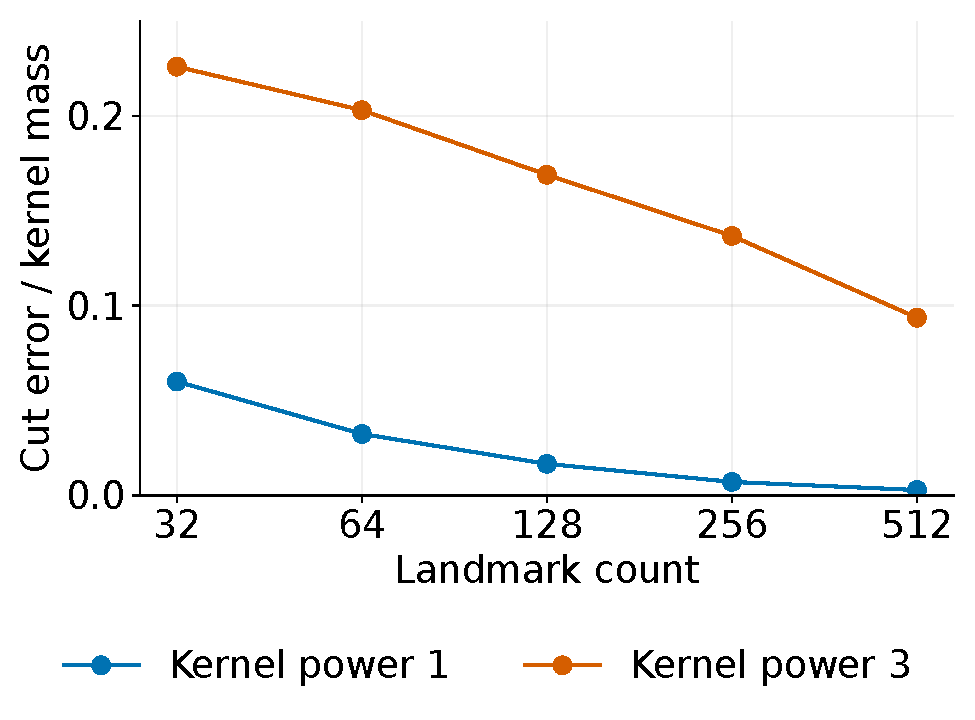
\includegraphics[width=6.5in]{systematic/fidelity.pdf}
\caption{Current-code cut fidelity. Each point is the largest absolute
factor-versus-exact cut difference divided by the corresponding kernel's
off-diagonal mass, over six full datasets, three factor seeds and five
partitions. Each set contains the returned partition and four count-preserving
perturbations. The ordinary and cubed kernels have different denominators.
These are observed cut errors, not uniform approximation guarantees.}
\label{fig:current-fidelity}
\end{figure}

Grouping alone is an incomplete explanation for the method's separation.
With the entities, groups and exact fold counts fixed, factor-space optimization
improves both global overlap and mean nearest-training similarity on all six
datasets, relative to a seeded feasible assignment
(Table~\ref{tab:matched-groups}). Every group is preserved in these controls.
The experiment isolates an improvement available after grouping has already
been chosen; it does not attribute every advantage of the combined pipeline
to compression.

\begin{table}[htbp]\centering
\begin{tabular}{lrr}\toprule
Assignment & Global overlap / random & Mean nearest similarity\\\midrule
Feasible groups & 0.959 & 0.387\\
Groups + ordinary factor & 0.791 & 0.306\\
Groups + cubed factor & 0.745 & 0.292\\
\bottomrule\end{tabular}
\caption{Optimization beyond grouping. Every comparison retains the same entities, constructed groups and exact 80/10/10 counts. Values average six dataset means after averaging three seeds. The factor optimizer starts from the feasible control and preserves every group. Both optimized settings improve both measures on all six datasets. Lower values indicate less overlap.}
\label{tab:matched-groups}\end{table}

\FloatBarrier

Exact references distinguish approximation from optimization more directly.
On twenty 12-entity instances, we enumerate 2,970 admissible ungrouped
assignments and thirty assignments with paired entities as indivisible groups.
Even with all twelve landmarks, the heuristic has nonzero optimization gaps
on some ungrouped instances: the largest gaps are 0.0132 and 0.0408 of kernel
mass for the ordinary and cubed kernels. The grouped full-landmark cases reach
their enumerated optima in this small suite. Increasing rank can therefore
remove approximation error while leaving a separate optimization error.
The complete decomposition and accuracy--cost controls appear in the supplement.

\FloatBarrier
\subsection{Dense overlap and analogue exposure give different quality--cost choices}

The ordinary factor directly targets distributed overlap. Its mean global
score is \CurrentPlainGlobal{}, compared with \CurrentGraphGlobal{} for the
top-32 graph, after averaging seeds within each dataset.
The combined setting reduces nearest-training exposure relative to the plain
setting, while the top-32 graph achieves lower mean exposure than the combined
setting (\CurrentGraphNearest{} versus \CurrentCombinedNearest{}).
Changing graph degree also changes the available trade-off
(Figure~\ref{fig:current-quality}). These outcomes support choosing a
representation and objective for a specified boundary rather than expecting
one method ordering for every separation criterion.

\begin{figure}[htbp]
\centering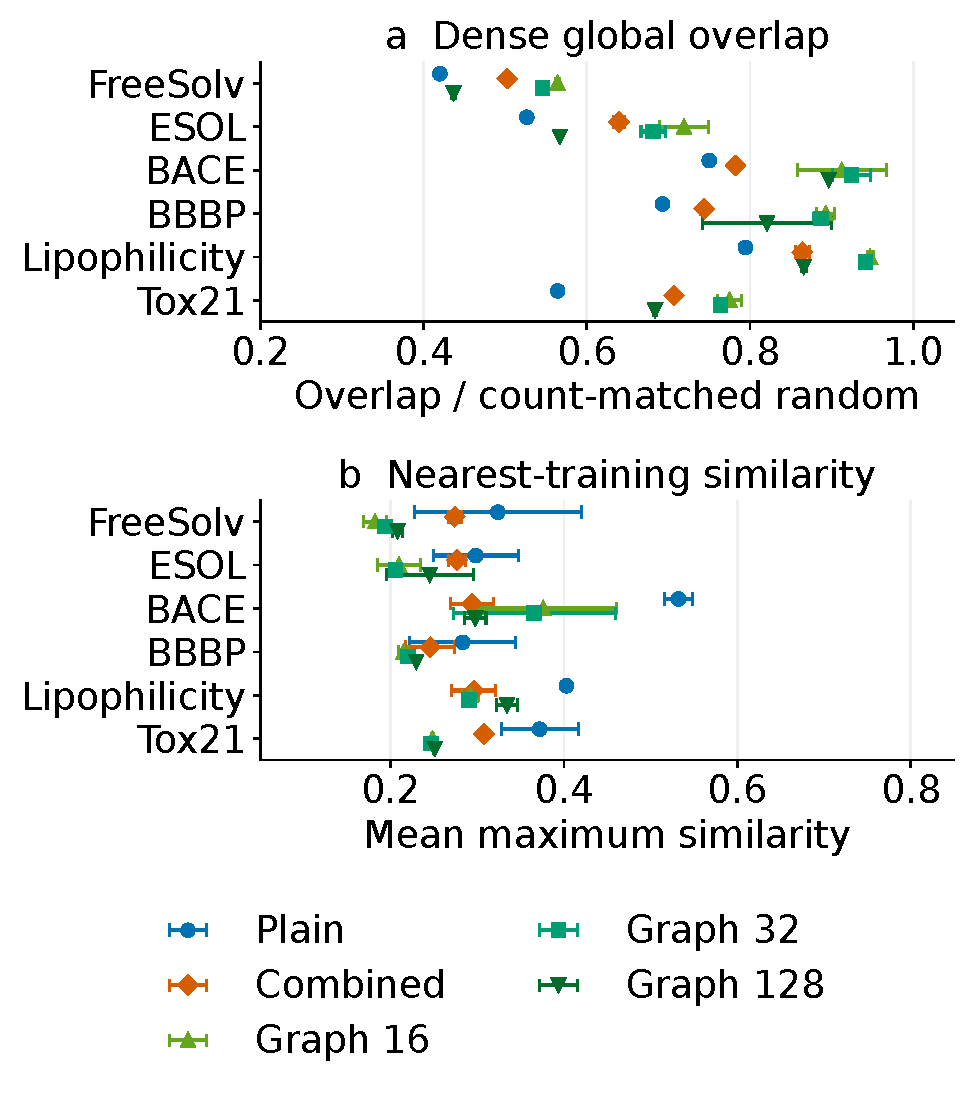
\includegraphics[width=6.5in]{systematic/quality.pdf}
\caption{Global and local quality for six full molecular datasets.
The primary global score is normalized by the analytic random expectation at
the actual counts; the local score is mean test-to-training maximum similarity.
Points average three split seeds and bars show their standard deviations.
All methods retain the same input entities and use a 1\% count corridor.
Graph labels identify ordinary pairwise degrees; graph construction and any
count repair are included in its runtime. All scores use the original ordinary
Tanimoto kernel. Lower values indicate less overlap.}
\label{fig:current-quality}
\end{figure}

DataSAIL provides the closer dense-objective comparison and reveals the
importance of admissible partitions. Sixteen of its twenty-four prespecified
configurations return assignments; eight report infeasibility under their
cluster and capacity settings. At exactly matched native counts, entity-level
low rank has mean global score \CurrentMatchedGlobal{}, versus
\CurrentNativeGlobal{} for DataSAIL. Requiring low rank to preserve the groups
passed to DataSAIL's solver changes its mean to
\CurrentMatchedGroupsGlobal{}, eliminating that average quality advantage.
These summaries weight the four datasets equally after averaging their
configurations.

Matching counts alone thus leaves a material difference in constraints.
Matching groups also leaves a distinction between linked cluster similarities
and sums over entity-level similarities, as well as different optimizers.
The comparison does not establish that compression solves an identical
optimization problem better. It establishes an economical way to construct
entity-level dense-overlap splits, with the consequences of additional
indivisibility constraints made visible. The supplement reports all native
outcomes, timings, group-preserving controls and memory profiles.

\FloatBarrier
\subsection{Exact capacities have a measurable computational cost}

At 100,000 ChEMBL fingerprints on two CPU cores, the median plain split-call
time is \CurrentExactCpuSeconds{} seconds with exact counts and
\CurrentCorridorCpuSeconds{} seconds with a 1\% corridor.
The inputs, rank and restart settings are otherwise matched.
The difference reflects the cost of feasible refinement, including the use of
swaps at exact capacities (Figure~\ref{fig:current-scaling}).
Linear factor storage therefore does not imply the same runtime at different
capacity tolerances.

On lambda13, the current plain implementation partitions two million
fingerprints in a median \CurrentLargeCpuSeconds{} seconds using 32 CPU cores,
with peak process RSS of \CurrentLargeCpuMemory{} GiB.
All three cases retain all entities and satisfy the declared 1\% corridor.
This is a separate hardware configuration from the paired two-core comparison;
the difference is not interpreted as an algorithmic speedup.

\begin{figure}[htbp]
\centering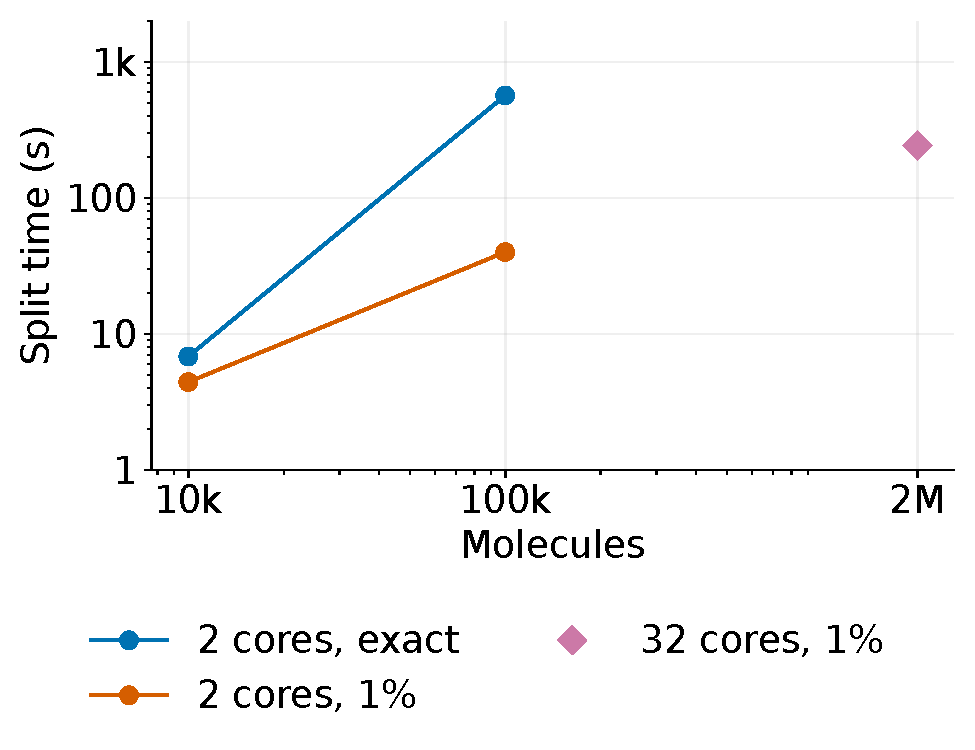
\includegraphics[width=6.5in]{systematic/cpu_scaling.pdf}
\caption{Current-code plain split-call time on nested ChEMBL samples, using
rank 256, four restarts and two refined candidates. Two-core cases run on lambda2;
the separate 32-core point runs on lambda13. Points are medians of completed cases.
Warm-up, feature loading and independent auditing
are outside the split clock. The full case inventory, including end-to-end
budget failures and the distinct combined-setting range, appears in the
supplement. An end-to-end failure is not assigned a split-call runtime.}
\label{fig:current-scaling}
\end{figure}

The large-data protocol checks quality as well as computational cost.
For every completed 100,000- and two-million-entity plain case, the independently
sampled returned-cut error interval has an upper endpoint below 0.008 of ordinary
kernel mass. Uniformly sampled test queries are also compared with every
training entity, rather than a subsampled training reference.
At two million entities, mean nearest-training similarity is
\CurrentLargeNearest{} across the three sets of sampled queries, showing that
low global overlap does not remove close-analogue exposure.
Sample sizes and conservative query-sampling intervals accompany the results.
The earlier v0.1 H100 measurements remain archival evidence and are not used
as timings of the current implementation.

\FloatBarrier
\subsection{Split usefulness depends on the transfer task}

Independent cohorts give a direct test of what an evaluation boundary predicts.
In the synthetic family model, random splitting identifies the better model
for known-family interpolation in all twenty generated instances, but identifies
the better model for new-family transfer in none. The combined split shows the
reverse pattern: agreement in all twenty new-family instances and none of the
interpolation instances. Plain splitting lies between these outcomes
(Figure~\ref{fig:current-deployment}).

\begin{figure}[htbp]
\centering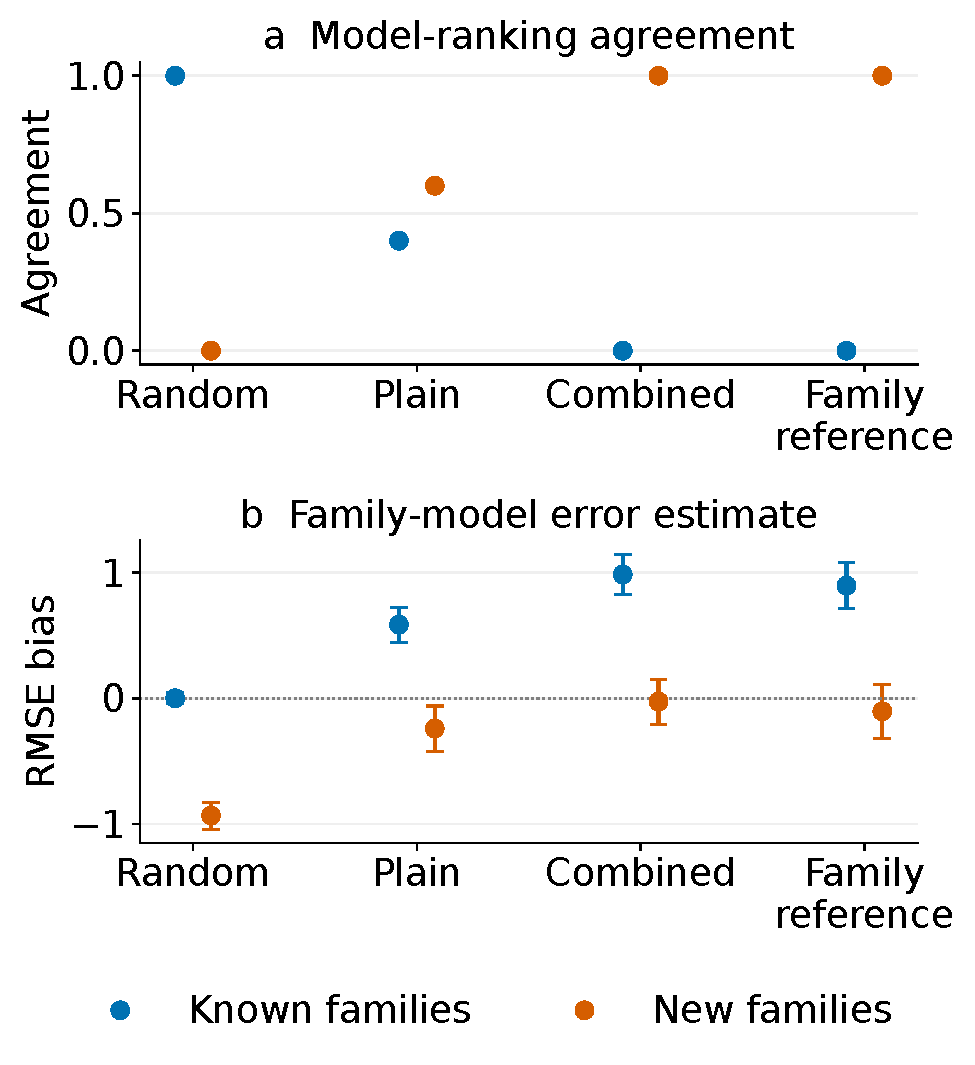
\includegraphics[width=6.5in]{systematic/deployment.pdf}
\caption{Evaluation boundaries for two transfer tasks in twenty synthetic
instances. (a) Agreement of held-out and independent-cohort model rankings.
(b) RMSE bias for the family-sensitive model; negative values are optimistic.
Bars are descriptive 95\% bootstrap intervals over instances.
Known-family cohorts condition on families present in training.
The family reference uses generator identities, and invariant ridge receives
the stable features. This mechanism test supplies no prospective validation.}
\label{fig:current-deployment}
\end{figure}

The direction of error is as relevant as the ranking. Random evaluation is
optimistic about the family-sensitive model on the new-family cohort, whereas
the combined split is pessimistic about that model's interpolation performance.
Stronger separation is useful when it matches the intended transfer boundary.
Its lower held-out score alone does not make it a more realistic test.

An earlier-release assay study illustrates a related risk in real molecular
data. Across ten prespecified external assays, the combined setting gives
mean random-forest ROC-AUC \ExtCombinedRF{}. A label-balance sensitivity intervention at
unchanged counts raises this to \ExtCombinedBalancedRF{}.
The intervention also changes structural composition and may break groups,
so it cannot isolate a causal contribution of label proportions.
These archival results demonstrate why target composition and absolute
predictive scores should accompany similarity measures. They supply no
observed future outcomes against which to validate a deployment claim.
